本研究で開発した2脚ロボットの外観をFig.\ref{robot_outline}に示す.
ロボットの大きさは,高さ510*幅230*奥行き140[mm],重量2.5[kg]であり,股関節にロールとピッチ方向,膝関節と距腿関節にピッチ方向の自由度をもつ.
股関節の2自由度は,ROBOTIS社製Dynamixel xのサーボモータ(Fig.\ref{dynamixel})によって駆動される.また,膝関節と距腿関節は,マッキベン型空気圧人工筋(Fig.\ref{muscle})(以下,空気圧人工筋と呼ぶ)によって駆動される.

ここで,膝関節と距腿関節のアクチュエータに空気圧人工筋を使用する理由は,空気圧人工筋によって生み出される関節の柔軟性を生かして,走行時のSLIPモデルにおけるばね要素を再現することができると考えたためである.
また,股関節に空気圧人工筋ではなくサーボモータを使用する理由は,股関節,特にロール軸のコンプライアンスを小さくすることが必要であり,空気圧人工筋では必要な剛性を出すことが難しいためである.

股関節と膝関節,膝関節と距腿関節の間隔は200[mm]で統一しており,股関節同士の間隔は50[mm]としている.
本研究において,使用しているサーボモータは,制御周期20[msec]で角度制御を行っている.
空気圧人工筋は,外部のエアコンプレッサによって空気を供給しており,最大で600[kPa]給気することが可能である.
空気量を調節する弁にはオンオフ弁(SMC,Fig.\ref{valve})を使用し,圧力センサを使用することで圧力制御を行うことが可能である.



\begin{figure}[htbp]
 \centering
 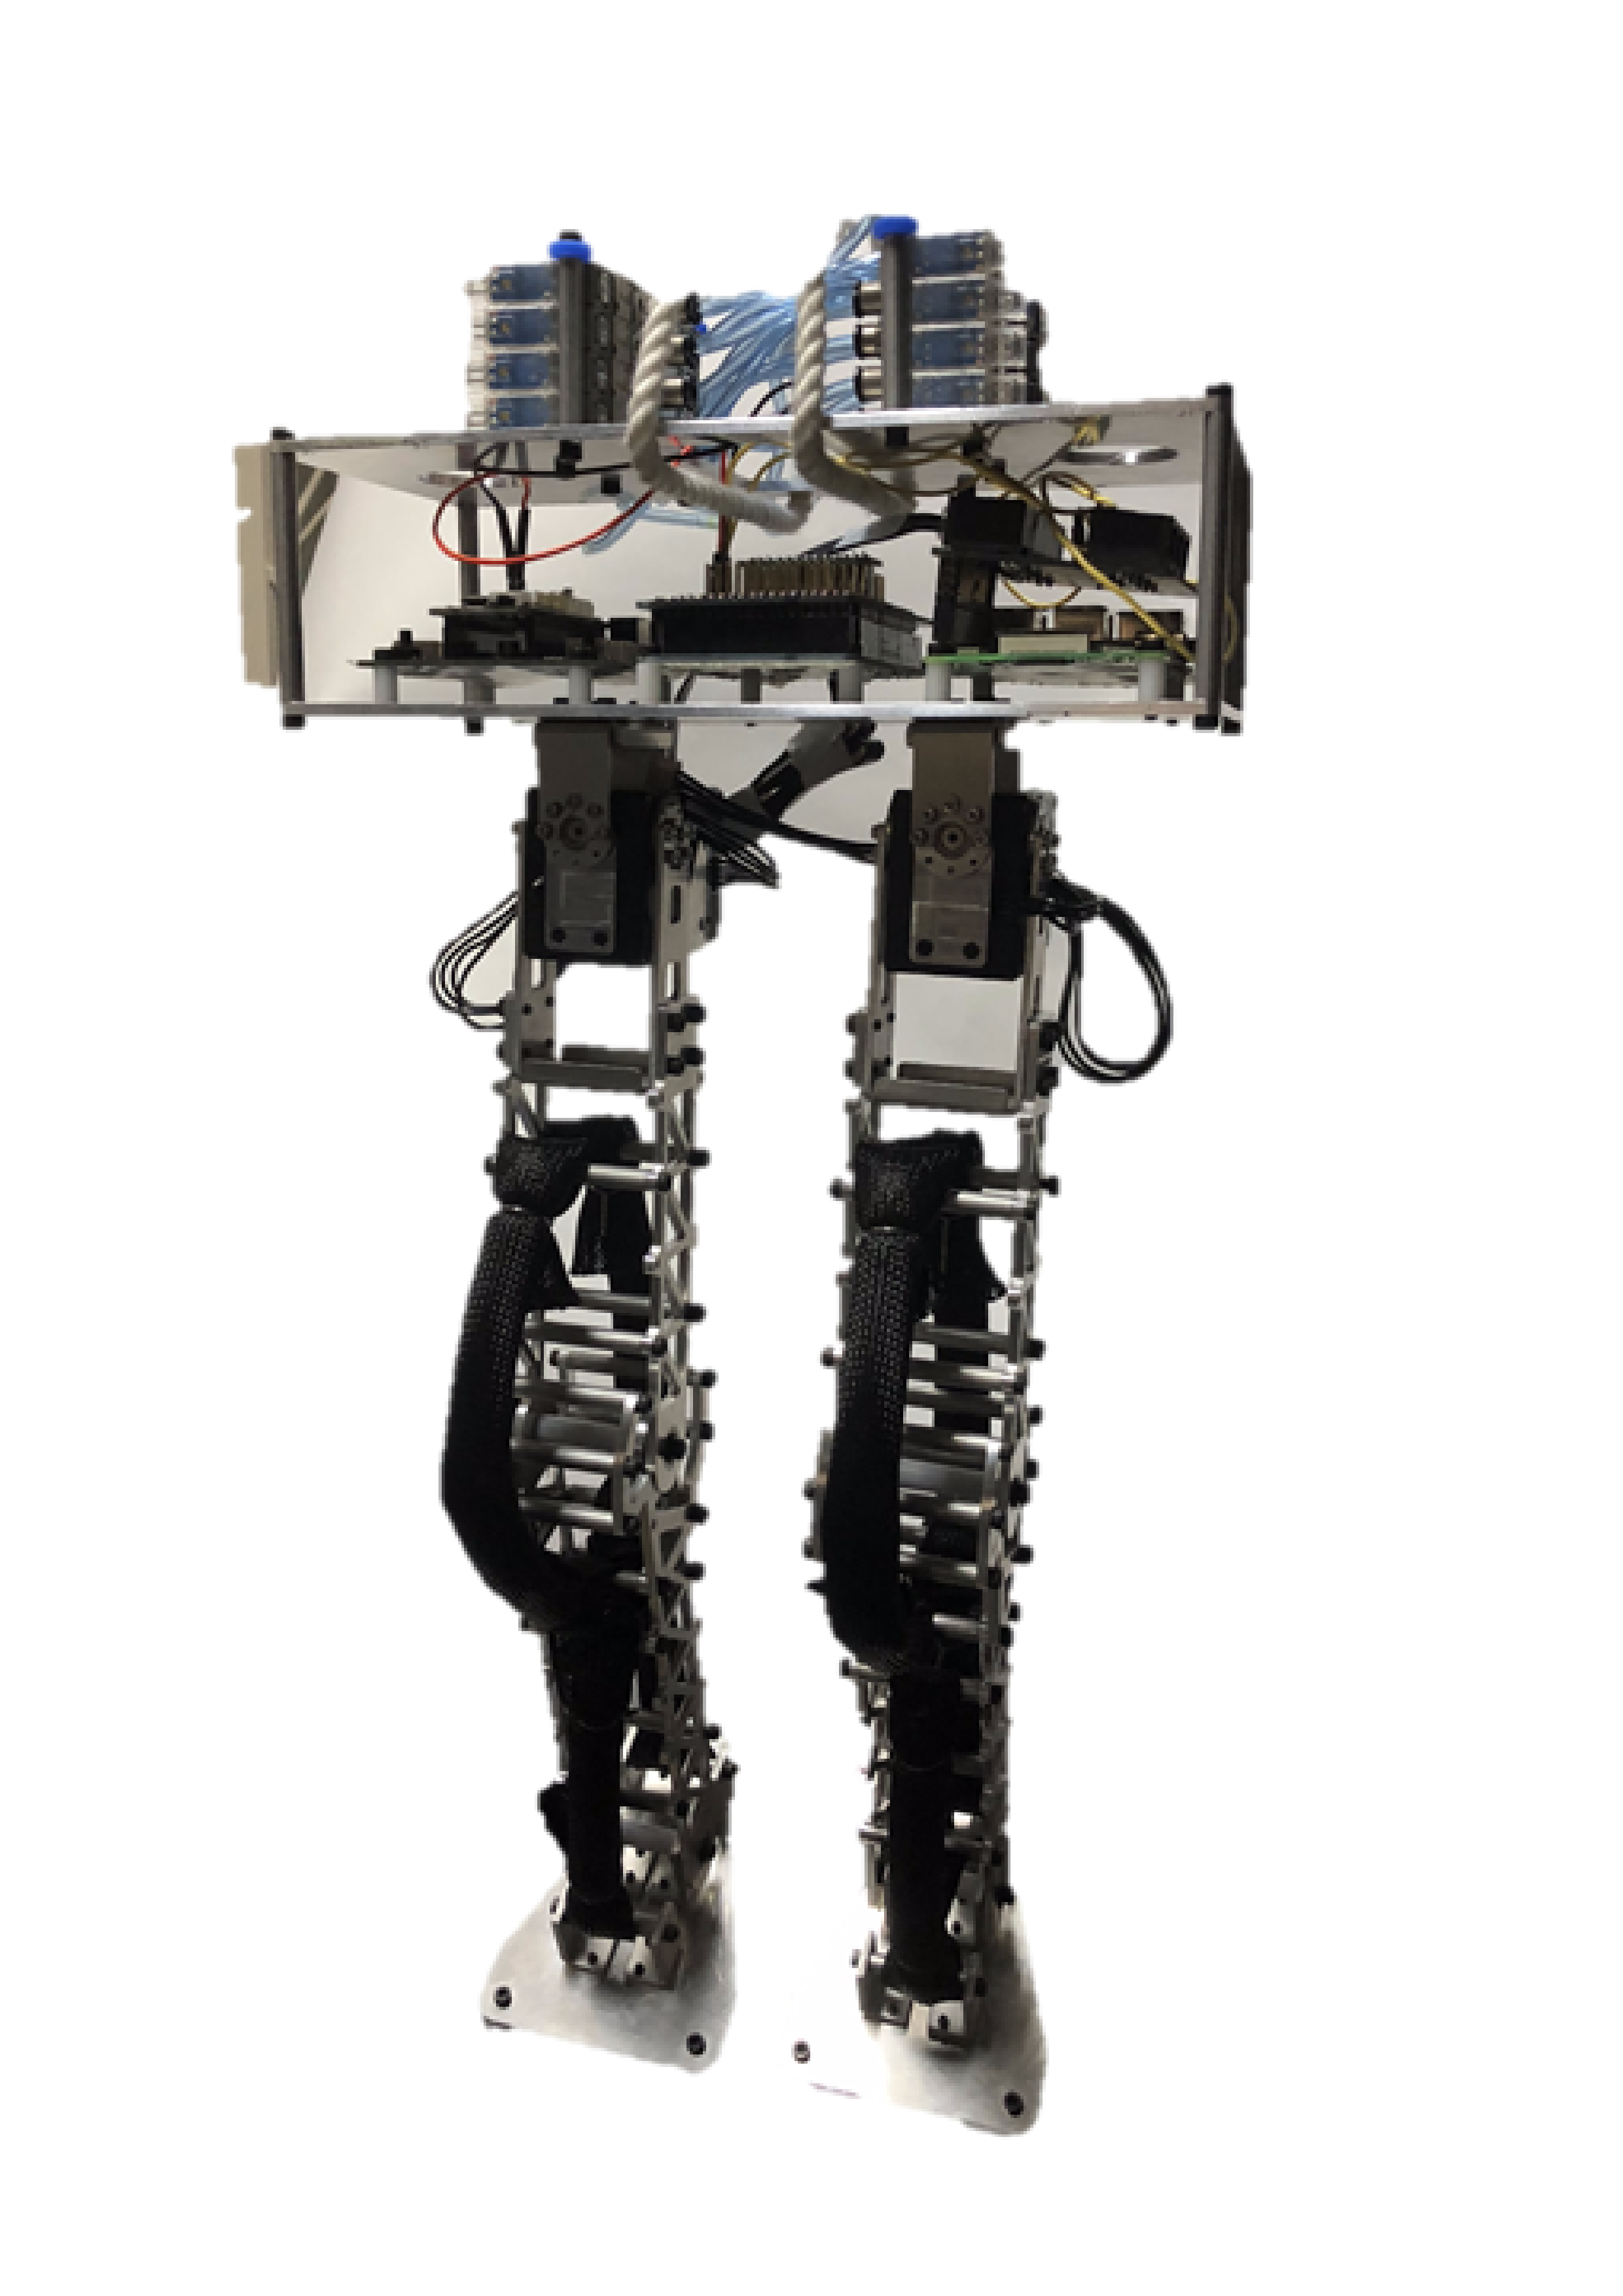
\includegraphics[clip,width=8.5cm]{./fig/robot.JPG}
    \caption{ロボットの外観.\label{robot_outline}}
\end{figure}

\begin{figure}
  \begin{minipage}[b]{.5\hsize}
   \centering
   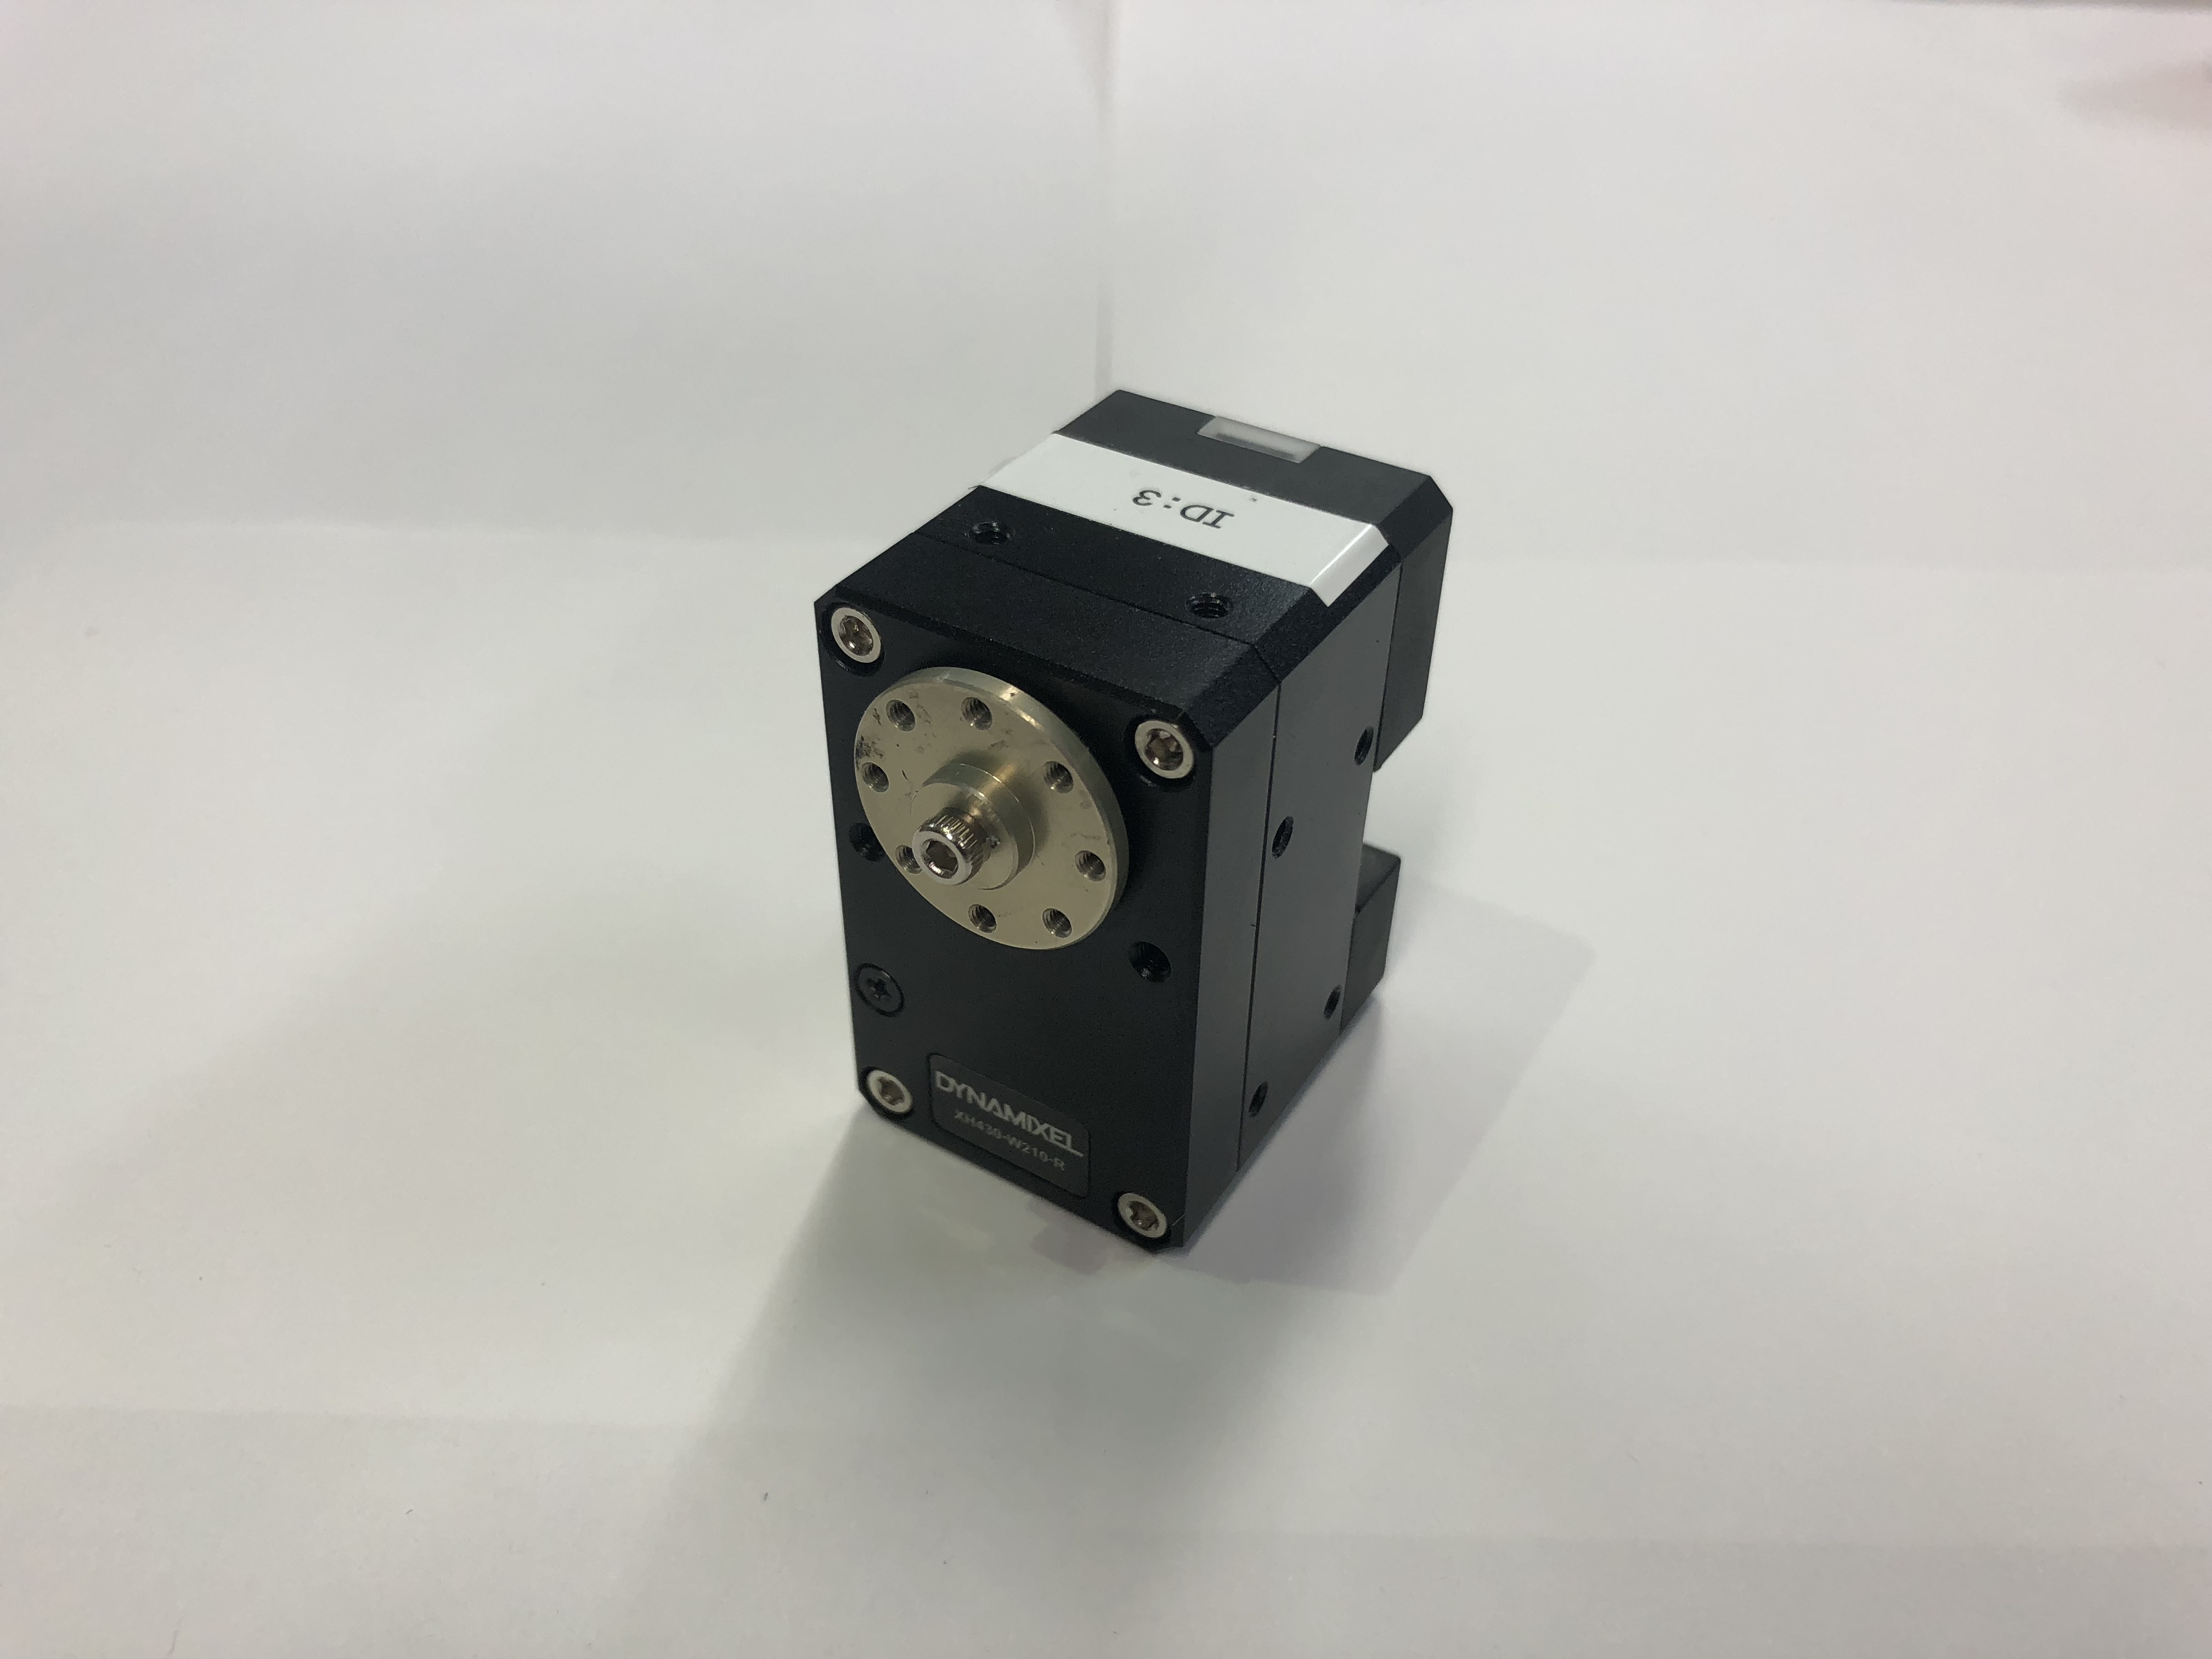
\includegraphics[clip,width=5.0cm]{./fig/dynamixel.JPG}
   \subcaption{ロボットに使用するサーボモータDynamixel x.\label{dynamixel}}
  \end{minipage}
  \begin{minipage}[b]{.5\hsize}
   \centering
   \includegraphics[clip,width=6.0cm]{./fig/McKibben.png}
   \subcaption{ロボットに使用するマッキベン型空気圧人工筋.\label{muscle}}
  \end{minipage}
  \caption{アクチュエータ.\label{actuator}}
\end{figure}

\begin{figure}[htbp]
 \centering
 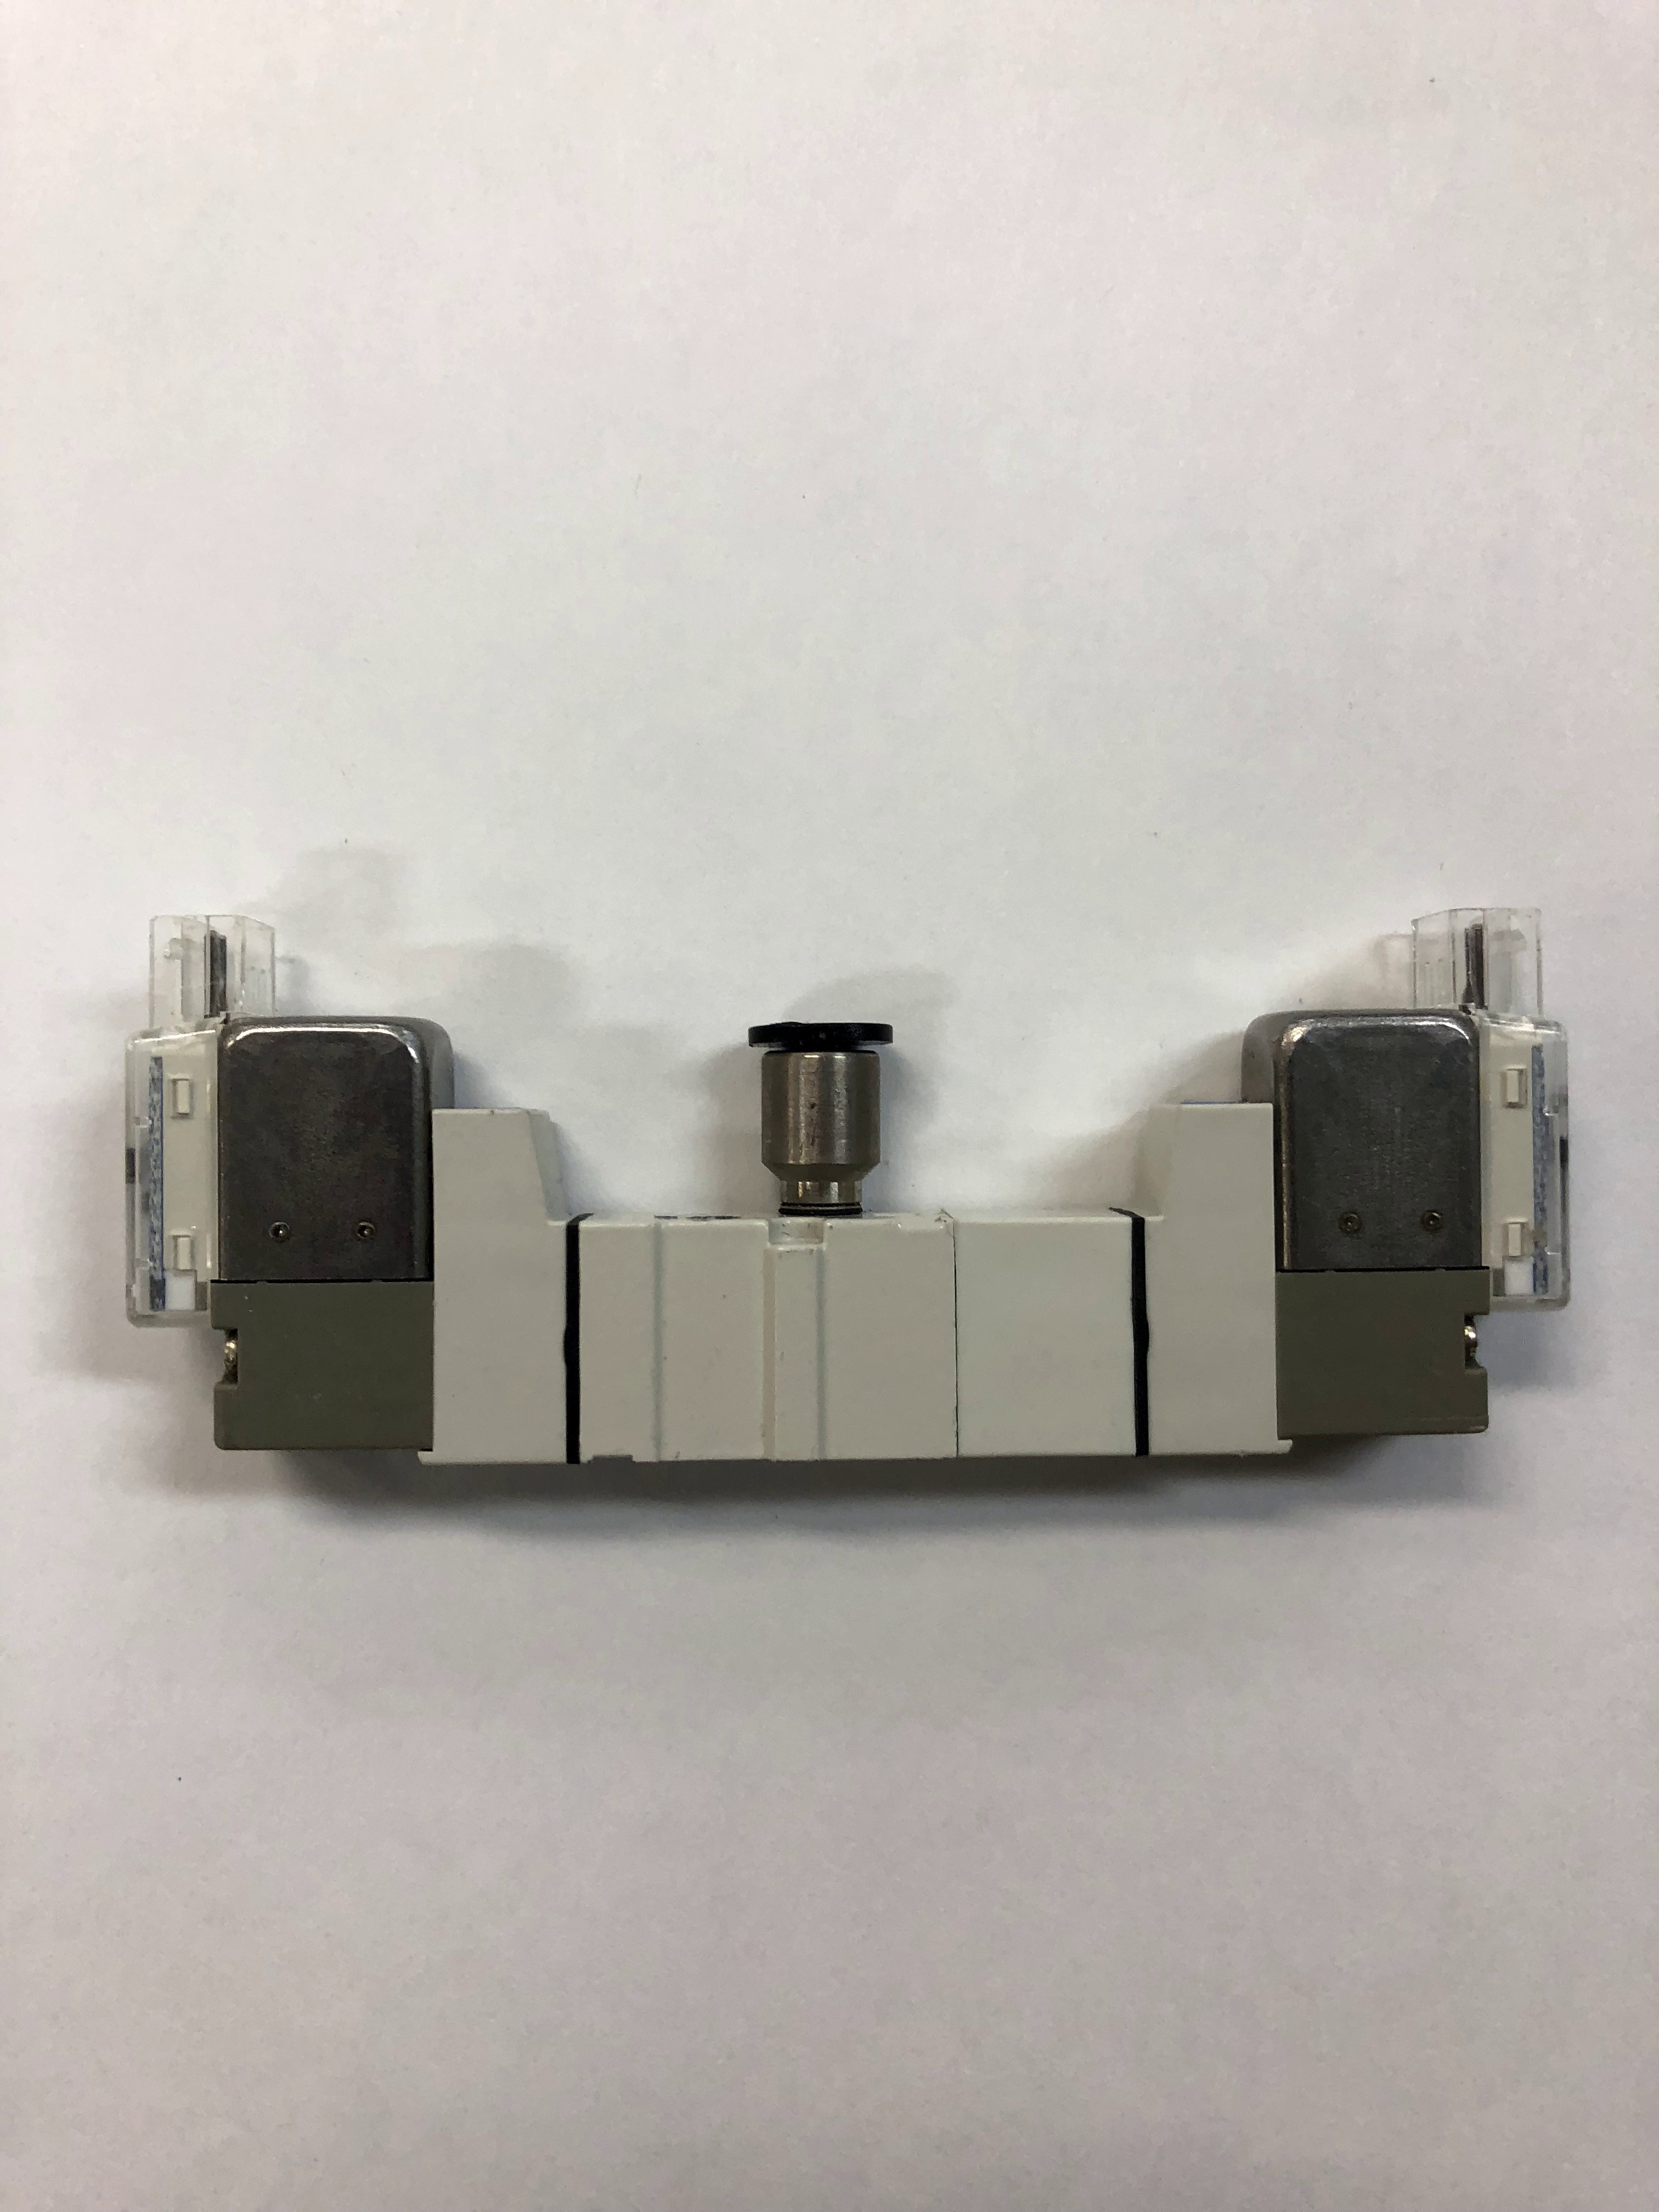
\includegraphics[clip,width=4.0cm]{./fig/valve.JPG}
    \caption{使用するオンオフ電磁弁.\label{valve}}
\end{figure}


\subsection{空気圧人工筋の拮抗駆動}
空気圧人工筋をアクチュエータに使用することによる利点の1つが,拮抗駆動による剛性調節機能である.
Fig.\ref{stiffness}に示すように,空気圧人工筋を関節に拮抗配置し,対になった筋に空気を給排気すると,その関節を伸展又は屈曲させることができる.
このとき,拮抗配置された2つの空気圧人工筋の内圧を低くすると,弾性係数が低くなるために,関節の剛性は低くなる.
逆に,空気圧人工筋の内圧を高くすると,弾性係数は高くなり,関節の剛性は高くなる.
このように,対になった空気圧人工筋の内圧を変化させることによって,一定範囲の関節角であれば,関節角を変化させずに関節の剛性を変化させることができる.
本研究では,歩行時には関節の剛性が高く,走行時には関節の剛性がある程度低い状態が求められるため,空気圧人工筋を拮抗駆動した場合に生じるこの現象は,提案したモデルの再現に有用であると考えられる.

\begin{figure}[htbp]
 \begin{minipage}[b]{.5\linewidth}
 \centering
 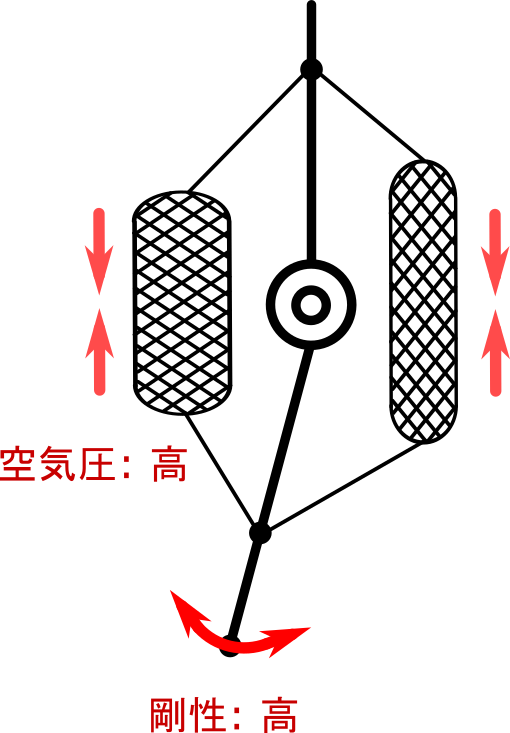
\includegraphics[width = 6.0cm, clip]{./fig/pair_high.png}
 \end{minipage}
 \begin{minipage}[b]{.5\linewidth}
 \centering
 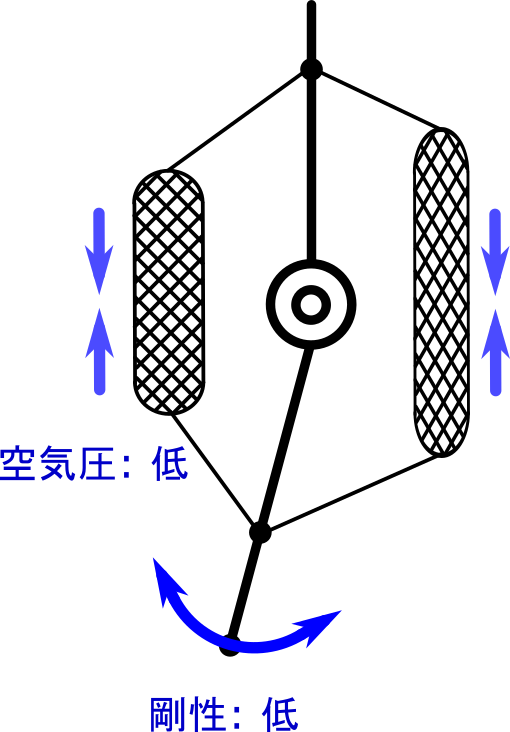
\includegraphics[width = 6.0cm,clip]{./fig/pair_low.png}
 \end{minipage}
 \caption{空気圧人工筋の拮抗駆動の構成.\label{stiffness}}
\end{figure}


\subsection{筋配置}
本研究で使用するロボットには,片脚で4本,合計で8本の空気圧人工筋を使用している.
各人工筋のチューブ径はφ6[mm]であり,長さは,\#0中間広筋は150[mm],\#1膝窩筋は120[mm],\#2前脛骨筋と\#3ヒラメ筋は50[mm]である.

これらの筋は,ヒトの身体における単関節筋の役割と構造を有している.
一方,このロボットは,ヒトの下半身に存在する多関節筋は実装していない.
その理由は,モータを使用している股関節に関して,空気圧人工筋とモータを両立させて使用することは困難であるためである.
また,空気圧人工筋のみによって駆動されている膝関節と距腿関節に関しても,制御を簡単化できるため,多関節筋を省略している.

\begin{figure}[htbp]
 \centering
 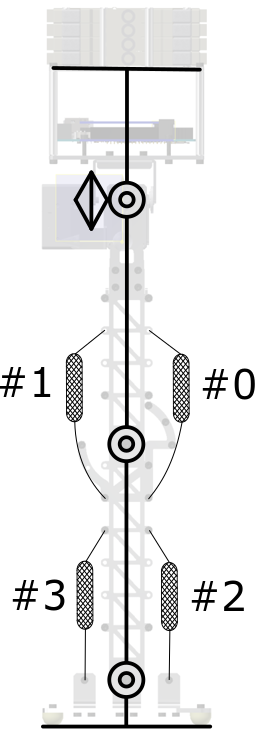
\includegraphics[clip,width=3.0cm]{./fig/robot_cad_muscle.png}
    \caption{ロボットの筋配置.\label{muscle_placement}}
\end{figure}

\begin{table}[htbp]
 \centering
 \begin{tabular}{|l||c|c|c|} \hline
    No. & 筋 & 機能 & 長さ\\ \hline \hline
    \#0 & 中間広筋 & 膝関節伸展 & 150mm \\
    \#1 & 膝窩筋 & 膝関節屈曲 & 120mm \\
    \#2 & 前脛骨筋 & 距腿関節背屈 & 50mm \\
    \#3 & ヒラメ筋 & 距腿関節屈曲 & 50mm \\ \hline
 \end{tabular}
\end{table}




\subsection{回路構成}
本ロボットの回路構成をFig.\ref{circuit}に示す.
ロボットの動作指令を送るマスタにはRaspberryPi3(Fig.\ref{raspi})を,空気圧人工筋に使用する電磁弁の操作には,Arduino DUE(Fig.\ref{due})を使用している.
これら2つのコントローラには,当研究室で開発されたシールド(Fig.\ref{r_shield}, Fig.\ref{d_shield})を併用し,LANケーブルで接続することで,シリアル通信でデータの送受信を行っている.
また,モータの操作には,ROBOTIS社製のUSB通信コンバータであるU2D2(Fig.\ref{u2d2})を使用し,マスタから直接データの送受信を行っている.

 \begin{figure}
  \begin{minipage}[b]{.45\hsize}
   \centering
   \includegraphics[width=0.5\linewidth,clip]{./fig/raspi3.png} 
   \subcaption{マスタコントローラRaspberryPi3.\label{raspi}}
  \end{minipage}
  \begin{minipage}[b]{.45\hsize}
   \centering
   \includegraphics[width=0.5\linewidth,clip]{./fig/raspi3_board.png}
   \subcaption{Raspberrypi3に使用するシールド.\label{r_shield}}
  \end{minipage}
  \caption{マスタコントローラ.\label{master}}
  \begin{minipage}[b]{.45\hsize}
   \centering
   \includegraphics[width = .45\linewidth, clip]{./fig/arduinodue.png}
   \subcaption{スレーブコントローラArduinoDUE.\label{due}}
  \end{minipage}
  \begin{minipage}[b]{.45\hsize}
   \centering
   \includegraphics[width = 0.45\linewidth,clip]{./fig/arduino_board.png}
   \subcaption{ArduinoDUEに使用するシールド.\label{d_shield}}
  \end{minipage}
  \caption{スレーブコントローラ.\label{slave}}
 \end{figure}

\begin{figure}[htbp]
 \centering
 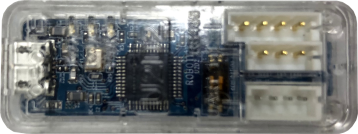
\includegraphics[clip,width = 5cm]{./fig/u2d2.png}
    \caption{サーボモータのUSB通信コンバータU2D2.\label{u2d2}}
\end{figure}

\begin{figure}[htbp]
 \centering
 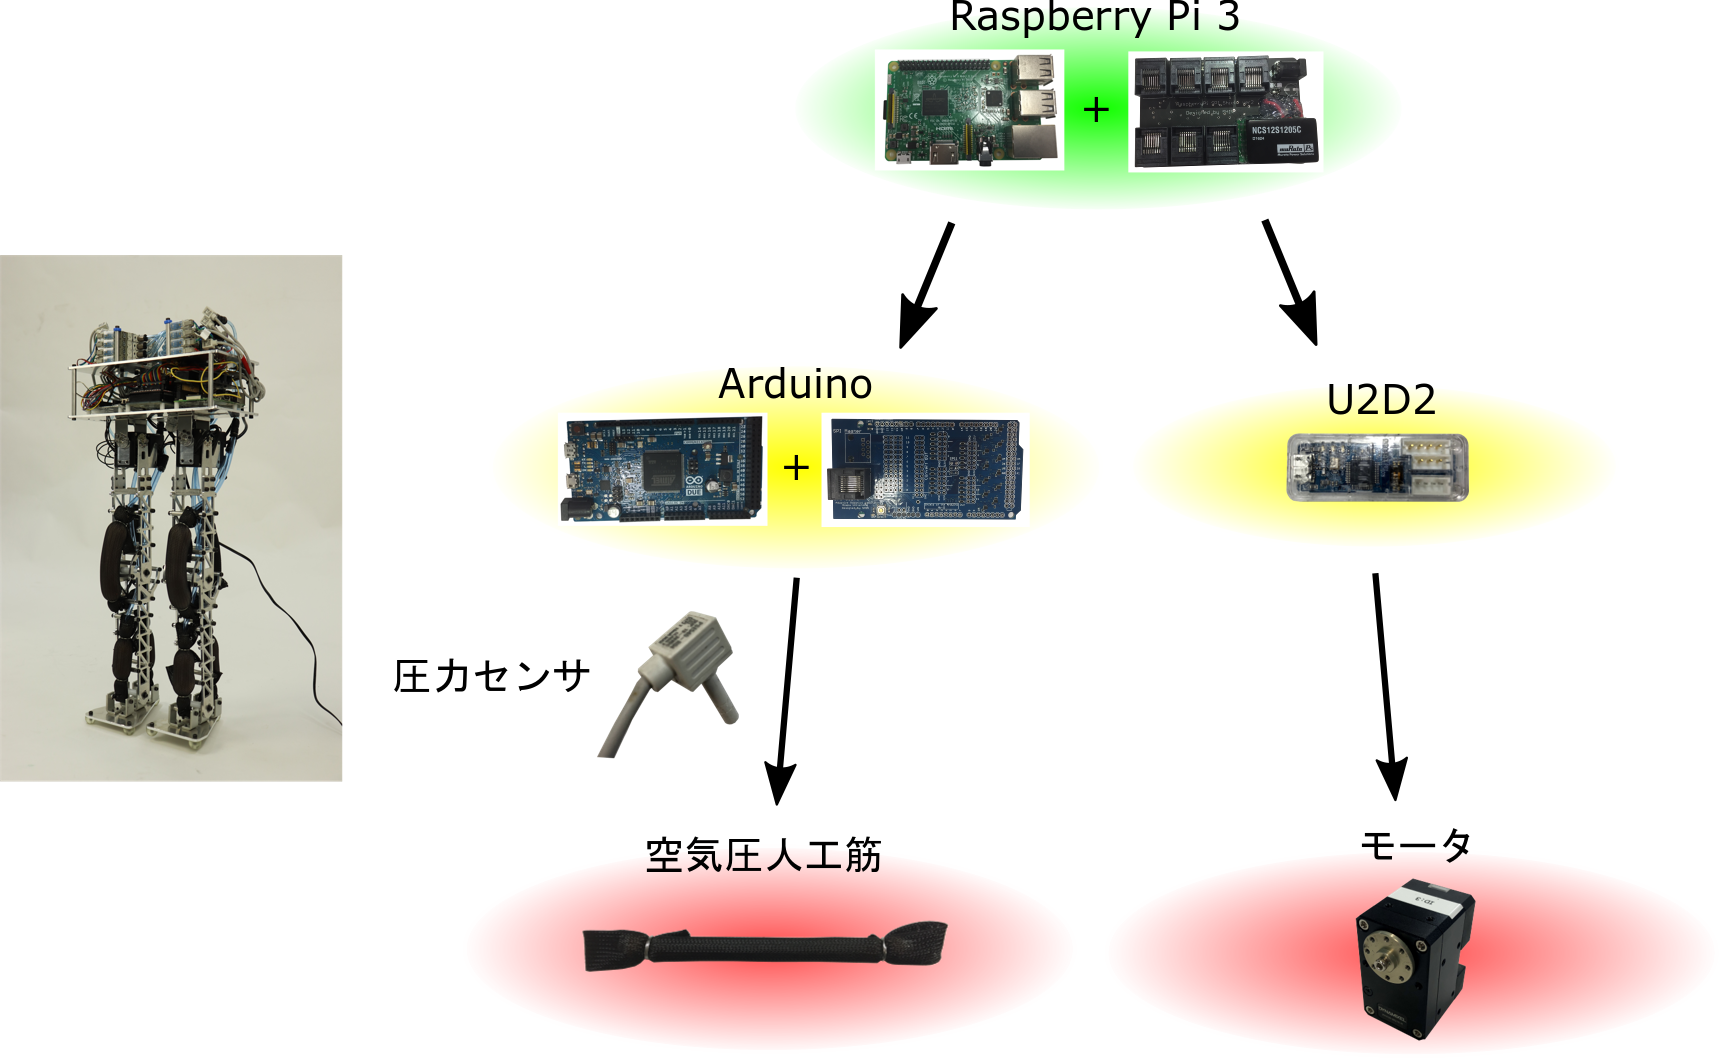
\includegraphics[clip,width = 16cm]{./fig/system.png}
    \caption{システム構成.\label{circuit}}
\end{figure}



\subsection{圧力制御}
本ロボットには,電磁弁と空気圧人工筋の間に,圧力センサ(SMC,PSE540-R04)(Fig.\ref{psensor})を配置しており,空気圧人工筋に給気する空気圧の計測を行うことができる.
このセンサ値と目標値との差に応じて電磁弁を開閉することによって,圧力制御が可能である.
空気圧人工筋の出力が非線形性を持つことから,空気圧人工筋内の圧力値と関節角の関係を定式化することは困難であるため,事前に空気圧と関節角の対応を把握することは,実際の動作生成において有用であると考えられる.
そこで,本ロボットでの歩行実験を行う前に,圧力制御を利用し,関節ごとに空気圧人工筋内の圧力値と関節角の対応を調べた.
Fig.\ref{ankle},Fig.\ref{knee}にその対応を表した図を示す.
横軸は伸展側の空気圧人工筋内の圧力値,縦軸は屈曲側の空気圧人工筋内の圧力値であり,グラフは,それぞれの圧力値に対する関節角を示している.
Fig.\ref{ankle}では,背屈の場合を+,足部と下腿が垂直である状態を0,底屈の場合を-で表しており,Fig.\ref{knee}では,伸展状態を0[deg],屈曲を+として関節角を表示している.

 \begin{figure}
  \begin{minipage}[b]{.5\linewidth}
   \centering
   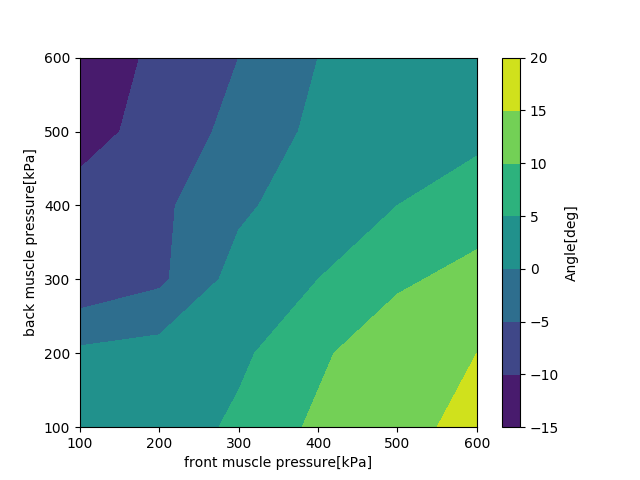
\includegraphics[clip,width = 9cm]{./fig/l_ankle_5deg.png}
   \subcaption{左脚距腿関節の対応\label{l_ankle}.}
  \end{minipage}
  \begin{minipage}[b]{.5\linewidth}
   \centering
   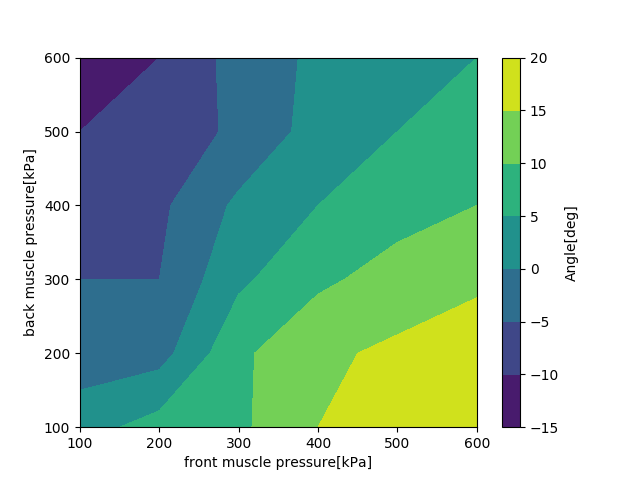
\includegraphics[clip,width = 9cm]{./fig/r_ankle_5deg.png}
   \subcaption{右脚距腿関節の対応\label{r_ankle}.}
  \end{minipage}
  \caption{空気圧人工筋内の圧力と距腿関節角度の対応.\label{ankle}}
  \begin{minipage}[b]{.5\linewidth}
   \centering
   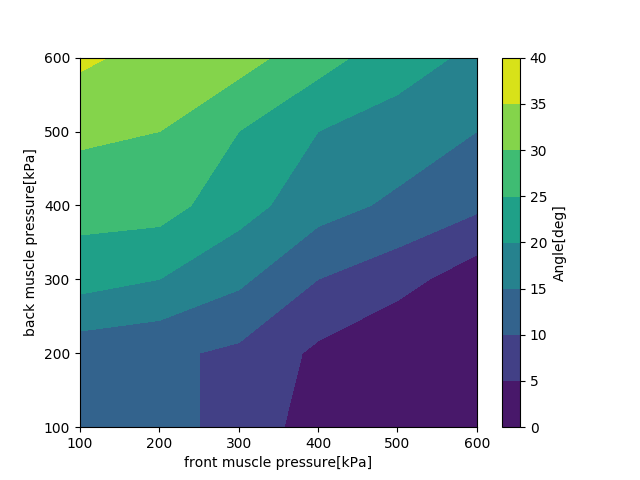
\includegraphics[clip,width = 9cm]{./fig/l_knee_5deg.png}
   \subcaption{左脚膝関節の対応\label{l_knee}.}
  \end{minipage}
  \begin{minipage}[b]{.5\linewidth}
   \centering
   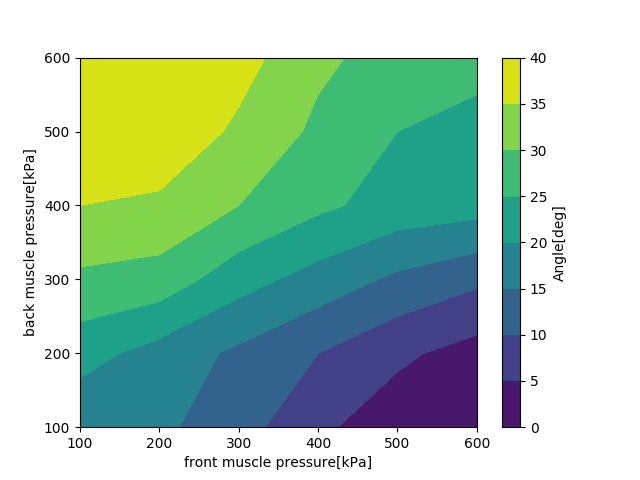
\includegraphics[clip,width = 9cm]{./fig/r_knee_5deg.png}
   \subcaption{右脚膝関節の対応\label{r_knee}.}
  \end{minipage}
  \caption{空気圧人工筋内の圧力と膝関節角度の対応.\label{knee}}
 \end{figure}


%%%%%% モデルとの比較(もしかしたら削除)
\subsection{モデルとの比較}
